%%%%%%%%%%%%%%%%%%%%%%%%%%%%%%%%%%%%%%%%%%%%%%%%%%%%%%%%%%%%%%%%%%%%%%%%%%%%%%%%%%%%%%%%%%%%%%%%%%%%%%%%%%%%%%%%%%%%%%%%%%%%%%%%%%%%%%%%%%%%%%%%%%%%%%%%%%%
% This is just an example/guide for you to refer to when submitting manuscripts to Frontiers, it is not mandatory to use frontiers.cls nor frontiers.tex  %
% This will only generate the Manuscript, the final article will be typeset by Frontier after acceptance.                                                 %
%                                                                                                                                                         %
% When submitting your files, remember to upload this *tex file, the pdf generated with it, and all the figures.
%%%%%%%%%%%%%%%%%%%%%%%%%%%%%%%%%%%%%%%%%%%%%%%%%%%%%%%%%%%%%%%%%%%%%%%%%%%%%%%%%%%%%%%%%%%%%%%%%%%%%%%%%%%%%%%%%%%%%%%%%%%%%%%%%%%%%%%%%%%%%%%%%%%%%%%%%%%

%%% Version 2.4 Generated 2014/03/12 %%%
%%% You will need to have the following packages installed: datetime, fmtcount, etoolbox, fcprefix, which are normally inlcuded in WinEdt. %%%
%%% In http://www.ctan.org/ you can find the packages and how to install them, if necessary. %%%

\documentclass{frontiersENG} % for Engineering articles
%\documentclass{frontiersSCNS} % for Science articles
%\documentclass{frontiersHLTH} % for Health articles
%\documentclass{frontiersFPHY} % for Physics articles

%\setcitestyle{square}
\usepackage{url,lineno}
\linenumbers

% Leave a blank line between paragraphs in stead of using \\

\copyrightyear{}
\pubyear{}

\def\journal{Bioengineering}%%% write here for which journal %%%
\def\DOI{}
\def\articleType{Research Article}
\def\keyFont{\fontsize{8}{11}\helveticabold }
\def\firstAuthorLast{Sample {et~al.}} %use et al only if is more than 1 author
\def\Authors{First Author\,$^{1,*}$, Co-Author\,$^{2}$ and Co-Author\,$^2$}
% Affiliations should be keyed to the author's name with superscript numbers and be listed as follows: Laboratory, Institute, Department, Organization, City, State abbreviation (USA, Canada, Australia), and Country (without detailed address information such as city zip codes or street names).
% If one of the authors has a change of address, list the new address below the correspondence details using a superscript symbol and use the same symbol to indicate the author in the author list.
\def\Address{$^{1}$Laboratory X, Institute X, Department X, Organization X, City X , State XX (only USA, Canada and Australia), Country X \\
$^{2}$Laboratory X, Institute X, Department X, Organization X, City X , State XX (only USA, Canada and Australia), Country X  }
% The Corresponding Author should be marked with an asterisk
% Provide the exact contact address (this time including street name and city zip code) and email of the corresponding author
\def\corrAuthor{corresponding Author}
\def\corrAddress{Laboratory X, Institute X, Department X, Organization X, Street X, City X , State XX (only USA, Canada and Australia), Zip Code, X Country X}
\def\corrEmail{email@uni.edu}

% \color{FrontiersColor} Is the color used in the Journal name, in the title, and the names of the sections.


\begin{document}
\onecolumn
\firstpage{1}

\title[Running Title]{Article Title}
\author[\firstAuthorLast ]{\Authors}
\address{}
\correspondance{}
\extraAuth{}% If there are more than 1 corresponding author, comment this line and uncomment the next one.
%\extraAuth{corresponding Author2 \\ Laboratory X2, Institute X2, Department X2, Organization X2, Street X2, City X2 , State XX2 (only USA, Canada and Australia), Zip Code2, X2 Country X2, email2@uni2.edu}
\topic{}% If your article is part of a Research Topic, please indicate here which.

\maketitle

%%%%%%%%%%%%%%%%%%%%%%%%%%%%%%%%%%%%%%%%%%%%%%%%%%%%%%%%%%%%%%%%%%%%%%%%%%%%%%%%%%%%%%%%%%%%%%%%%%%%%%%%%%%%%%%%%%%%%%%%%%%%%%%%%%%%%%%%%%%%%%%%%%%%%%%%%%%%%%%%%%%%%%%%%%%%%%%%%%%%%%%%%%%%%%%%%%%%%%%%%%%%%%%%%%%%%%%%%%%%%%%%%%%%%%%
%%% The sections below are for reference only.
%%%
%%% For Original Research Articles, Clinical Trial Articles, and Technology Reports the section headings should be those appropriate for your field and the research itself. It is recommended to organize your manuscript in the
%%% following sections or their equivalents for your field:
%%% Abstract, Introduction, Material and Methods, Results, and Discussion.
%%% Please note that the Material and Methods section can be placed in any of the following ways: before Results, before Discussion or after Discussion.
%%%
%%%For information about Clinical Trial Registration, please go to http://www.frontiersin.org/about/AuthorGuidelines#ClinicalTrialRegistration
%%%
%%% For Clinical Case Studies the following sections are mandatory: Abstract, Introduction, Background, Discussion, and Concluding Remarks.
%%%
%%% For all other article types there are no mandatory sections.
%%%%%%%%%%%%%%%%%%%%%%%%%%%%%%%%%%%%%%%%%%%%%%%%%%%%%%%%%%%%%%%%%%%%%%%%%%%%%%%%%%%%%%%%%%%%%%%%%%%%%%%%%%%%%%%%%%%%%%%%%%%%%%%%%%%%%%%%%%%%%%%%%%%%%%%%%%%%%%%%%%%%%%%%%%%%%%%%%%%%%%%%%%%%%%%%%%%%%%%%%%%%%%%%%%%%%%%%%%%%%%%%%%%%%%%

\begin{abstract}

%%% Leave the Abstract empty if your article falls under any of the following categories: Editorial Book Review, Commentary, Field Grand Challenge, Opinion or specialty Grand Challenge.
\section{}
%As a primary goal, the abstract should render the general significance and conceptual advance of the work clearly accessible to a broad readership. References should not be cited in the abstract.
Refer to \\ \url{http://www.frontiersin.org/}\texttt{\journal}\url{/authorguidelines} \\ or \textbf{Table\ref{Tab:01}} for abstract requirement and length according to article type.


\tiny
 \keyFont{ \section{Keywords:} Text Text Text Text Text Text Text Text } %All article types: you may provide up to 8 keywords; at least 5 are mandatory.
\end{abstract}

\section{Introduction}

% For Original Research Articles, Clinical Trial Articles, and Technology Reports the introduction should be succinct, with no subheadings.
%
% For Clinical Case Studies the Introduction should include symptoms at presentation, physical exams and lab results.
%
Text Text Text Text Text Text  Text Text Text Text Text Text Text Text Text  Text Text Text Text Text Text. Text Text Text Text Text Text  Text Text Text Text Text Text Text Text Text  Text Text Text Text Text Text. Text Text Text Text Text Text  Text Text Text Text Text Text Text Text Text  Text Text Text Text Text Text.Text Text Text Text Text Text  Text Text Text Text Text Text Text Text Text  Text Text Text Text Text Text.

%\begin{methods}
\section{Material \& Methods}

Text Text Text Text Text Text  Text Text Text Text Text Text Text Text Text  Text Text Text Text Text Text Text Text Text Text  Text Text Text Text Text Text  Text Text.  \cite{Neuro2013} might want to know about  text text text text Text Text Text Text  Text Text Text Text Text Text  Text Text. \citep{Gene2012} might want to know about  text text text text
Text Text Text Text Text Text  Text Text Text Text Text Text Text Text Text  Text Text Text Text Text Text Text Text Text Text  Text Text Text Text Text Text  Text Text.  \cite{Neurobot2013} might want to know about  text text text text

\begin{table}[!t]
\textbf{\refstepcounter{table}\label{Tab:01} Table \arabic{table}.}{ Maximum size of the Manuscript }

\processtable{ }
{\begin{tabular}{lllll}\toprule
 & Abstract max. legth (incl. spaces) & Figures or tables & Manuscript max. length & Final PDF length\\\midrule
Clinical Case Study & & & &\\
Clinical Trial & & & &\\
Hypothesis and Theory & & & &\\
Methods & 2000 characters  & 15 & 12000 words & 12 pages\\
Original Research & & & &\\
Review & & & &\\
Technology Report & & & &\\
Focused Review & 2000 characters & 5 & 5000 words & 5 pages\\
CPC &  1250 characters& 6 & 2500 words & 4 pages\\
Perspective & 1250 characters & 2 & 3000 words & 3 pages\\
Mini Review & & & &\\
Classification & 1250 characters & 10 & 2000 words & 12 pages\\
Editorial & none & none & 1000 words & 1 page \\
Book review & & & &\\
Frontiers Commentary & none & 1 & 1000 words & 1 page\\
General Commentary & & & &\\
Field Grand Challenge & & & &\\
Opinion & none & 1 & 2000 words & 2 pages\\
Specialty Grand Challenge& & & &\\\botrule
\end{tabular}}{}
\end{table}

Please note that very large tables (covering several pages) cannot be included in the final PDF for reasons of space. These tables will be published as supplementary material on the online article abstract page at the time of acceptance. The author will notified during the typesetting of the final article if this is the case. A link in the final PDF will direct to the online material.

\subsection{Original Research Articles, Clinical Trial Articles, and Technology Reports}

For Original Research Articles, Clinical Trial Articles, and Technology Reports the section headings should be those appropriate for your field and the research itself. It is recommended to organize your manuscript in the following sections or their equivalents for your field:

\begin{itemize}
%for bulleted list, use itemize
\item Introduction: Succinct, with no subheadings.
\item Materials and Methods: This section may be divided by subheadings. This section should contain sufficient detail so that when read in conjunction with cited references, all procedures can be repeated.
\item Results: This section may be divided by subheadings. Footnotes should not be used and have to be transferred into the main text.
\item Discussion: This section may be divided by subheadings. Discussions should cover the key findings of the study: discuss any prior art related to the subject so to place the novelty of the discovery in the appropriate context; discuss the potential short-comings and limitations on their interpretations; discuss their integration into the current understanding of the problem and how this advances the current views; speculate on the future direction of the research and freely postulate theories that could be tested in the future.
\end{itemize}

Please note that the Material and Methods section can be placed in any of the following ways: before Results, before Discussion or after Discussion.

\subsection{Clinical Case Studies}

For Clinical Case Studies the following sections are mandatory:

\begin{itemize}
%for bulleted list, use itemize
\item Introduction: Include symptoms at presentation, physical exams and lab results.
\item Background: This section may be divided by subheadings. Include history and review of similar cases.
\item Results: This section may be divided by subheadings. Include diagnosis and treatment.
\item Concluding Remarks
\end{itemize}

%\end{methods}



\section{Results}

Frontiers requires figures to be submitted individually, in the same order as they are referred to in the manuscript. Figures will then be automatically embedded at the bottom of the submitted manuscript. Kindly ensure that each table and figure is mentioned in the text and in numerical order. Permission must be obtained for use of copyrighted material from other sources (including the web). Please note that it is compulsory to follow figure instructions. Figures which are not according to the guidelines will cause substantial delay during the production process.

\begin{table}[!t]
\textbf{\refstepcounter{table}\label{Tab:02} Table \arabic{table}.}{ Resolution Requirements for the figures}

\processtable{}
{\begin{tabular}{lllll}\toprule
Image Type & Description & Format & Color Mode & Resolution\\\midrule
Line Art & An image composed of lines and text,  & TIFF, JPEG & RGB, Bitmap & 900 - 1200 dpi\\
           & which does not contain tonal or shaded areas.& & &\\
           Halftone & A continuous tone photograph, which contains no text. & TIFF, EPS, JPEG & RGB, Grayscale & 300 dpi\\
Combination & Image contains halftone + text or line art elements. & TIFF, JPEG & RGB,Grayscale & 600 - 900 dpi\\\botrule
\end{tabular}}{}
\end{table}

\begin{equation}
\sum x+ y =Z\label{eq:01}
\end{equation}

\textbf{Table\ref{Tab:02}} shows the resolution requirements for the figures. The figures must be legible:
\begin{enumerate}
\item The smallest visible text is no less than 8 points in height, when viewed at actual size.
\item Solid lines are not broken up.
\item Image areas are not pixelated or stair stepped.
\item Text is legible and of high quality.
\item Any lines in the graphic are no smaller than 2 points width.
\item The actual size of the figure must be of at least 8.5 cm.
\end{enumerate}

\section{Discussion}

Text Text Text Text Text Text  Text Text Text Text Text Text Text Text Text  Text Text Text Text Text Text Text Text Text Text.
Additional Requirements:
\subsection{Corrections}

Minor corrections to published articles can be communicated to the Frontiers Production Office at production.office@frontiersin.org. If you need to communicate important changes to an article please submit a General Commentary. Submit the article with the title “Erratum: Original Title of Article”.

\subsection{Commentaries on Articles}

At the beginning of your manuscript provide the citation of the article commented on.

\subsection{Focused Reviews}

For Tier 2 invited Focused Reviews the sections Introduction, Material and Methods, Results, and Discussion are recommended. In addition the authors must submit a short biography of the corresponding author(s). This short biography has a maximum of 600 characters, including spaces.

A picture (5 x 5 cm, in *.tif or *.jpg, min 300 dpi) must be submitted along with the biography in the manuscript and separately during figure upload.
Focused Reviews highlight and explain key concepts of your work. Please highlight a minimum of four and a maximum of ten key concepts in bold in your manuscript and provide the definitions/explanations at the end of your manuscript under “Key Concepts”. Each definition has a maximum of 400 characters, including spaces.

\subsection{Human Search and Animal Research}

All experiments on live vertebrates or higher invertebrates must be performed in accordance with relevant institutional and national guidelines and regulations. In the manuscript, authors must identify the committee approving the experiments and must confirm that all experiments conform to the relevant regulatory standards. For manuscripts reporting experiments on human subjects, authors must identify the committee approving the experiments and must also include a statement confirming that informed consent was obtained from all subjects. In Original Research Articles and Clinical Trial Articles these statements should appear in the Materials and Methods section.

\subsection{Clinical Trial Registration}

Clinical trials should be registered in a public trials registry in order to become the object of a publication at Frontiers. Trials must be registered at or before the start of patient enrollment. A clinical trial is defined as"any research study that prospectively assigns human participants or groups of humans to one or more health-related interventions to evaluate the effects on health outcomes."(\url{www.who.int/ictrp/en}). A list of acceptable registries can be found at \url{www.who.int/ictrp/en and www.icmje.org}.

\subsection{Inclusion of Proteomics Data}

Authors should provide relevant information relating to how the peptide/protein matches were undertaken, including methods used to process and analyze data, false discovery rates (FDR) for large-scale studies and threshold or cut-off rates for peptide and protein matches. Further information could include software used, mass spectrometer type, sequence database and version, number of sequences in database, processing methods, mass tolerances used for matching, variable/fixed modifications, allowable missed cleavages, etc.

Authors should provide as supplementary material information used to identify proteins and/or peptides. This should include information such as accession numbers, observed mass (m/z), charge, delta mass, matched mass, peptide/protein scores, peptide modification, miscleavages, peptide sequence, match rank, matched species (for cross species matching), number of peptide matches, ambiguous protein/peptide matches should be indicated, etc.
For quantitative proteomics analyses authors should provide information to justify the statistical significance including biological replicates, statistical methods, estimates of uncertainty and the methods used for calculating error.

For peptide matches with biologically relevant post-translational modifications (PTM) and for any protein match that has occurred using a single mass spectrum, authors should include this information as raw data, annotated spectra or submit data to an online repository (recommended option).
Authors are encouraged to submit raw or matched data and 2-DE images to public proteomics repositories. Submission codes and/or links to data should be provided within the manuscript.

\subsection{Data Sharing}

Frontiers supports the policy of data sharing, and authors are advised to make freely available any materials and information described in their article, and any data relevant to the article (while not compromising confidentiality in the context of human-subject research) that may be reasonably requested by others for the purpose of academic and non-commercial research. In regards to deposition of data and data sharing through databases, Frontiers urges authors to comply with the current best practices within their discipline.

\section*{Disclosure/Conflict-of-Interest Statement}
%Frontiers follows the recommendations by the International Committee of Medical Journal Editors (http://www.icmje.org/ethical_4conflicts.html) which require that all financial, commercial or other relationships that might be perceived by the academic community as representing a potential conflict of interest must be disclosed. If no such relationship exists, authors will be asked to declare that the research was conducted in the absence of any commercial or financial relationships that could be construed as a potential conflict of interest. When disclosing the potential conflict of interest, the authors need to address the following points:
%•	Did you or your institution at any time receive payment or services from a third party for any aspect of the submitted work?
%•	Please declare financial relationships with entities that could be perceived to influence, or that give the appearance of potentially influencing, what you wrote in the submitted work.
%•	Please declare patents and copyrights, whether pending, issued, licensed and/or receiving royalties relevant to the work.
%•	Please state other relationships or activities that readers could perceive to have influenced, or that give the appearance of potentially influencing, what you wrote in the submitted work.

The authors declare that the research was conducted in the absence of any commercial or financial relationships that could be construed as a potential conflict of interest.

\section*{Author Contributions}
%When determining authorship the following criteria should be observed:
%•	Substantial contributions to the conception or design of the work; or the acquisition, analysis, or interpretation of data for the work; AND
%•	Drafting the work or revising it critically for important intellectual content; AND
%•	Final approval of the version to be published ; AND
%•	Agreement to be accountable for all aspects of the work in ensuring that questions related to the accuracy or integrity of any part of the work are appropriately investigated and resolved.
%Contributors who meet fewer than all 4 of the above criteria for authorship should not be listed as authors, but they should be acknowledged. (http://www.icmje.org/roles_a.html)

The statement about the authors and contributors can be up to several sentences long, describing the tasks of individual authors referred to by their initials and should be included at the end of the manuscript before the References section.


\section*{Acknowledgement}
Text Text Text Text Text Text  Text Text Text Text Text Text Text Text  Text Text Text Text Text Text Text Text Text  Text Text Text.

\paragraph{Funding\textcolon} Text Text Text Text Text Text  Text Text.

\section*{Supplemental Data}
Text Text Text Text Text Text  Text Text Text Text Text Text Text Text Text  Text Text Text Text Text Text Text Text Text  Text Text Text.

\bibliographystyle{frontiersinSCNS&ENG} % for Science and Engineering articles
%\bibliographystyle{frontiersinHLTH&FPHY} % for Health and Physics articles
\bibliography{test}

\section*{Figures}

%%% Use this if adding the figures directly in the mansucript, if so, please remember to also upload the files when submitting your article
%%% There is no need for adding the file termination, as long as you indicate where the file is saved. In the examples below the files (logo1.jpg and logo2.eps) are in the Frontiers LaTeX folder
%%% If using *.tif files convert them to .jpg or .png

%\begin{figure}
%\begin{center}
%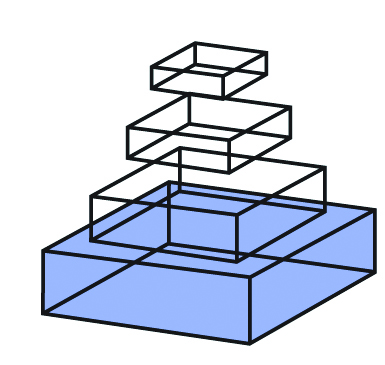
\includegraphics[width=3.5cm]{logo1}% This is a *.jpg file
%\end{center}
% \textbf{\refstepcounter{figure}\label{fig:01} Figure \arabic{figure}.}{ Enter the caption for your figure here.  Repeat as  necessary for each of your figures }
%\end{figure}

%\begin{figure}
%\begin{center}
%
\includegraphics[width=3.5cm]{logo2}% This is an *.eps file
%\end{center}
% \textbf{\refstepcounter{figure}\label{fig:02} Figure \arabic{figure}.}{ Enter the caption for your figure here.  Repeat as  necessary for each of your figures }
%\end{figure}

 \textbf{Figure 1.}{ Enter the caption for your figure here.  Repeat as  necessary for each of your figures.}\label{fig:01}% If you don't add the figures in the LaTeX files, please upload them when submitting the article.

%%% Frontiers will add the figures at the end of the provisional pdf automatically %%%

%%% The use of LaTeX coding to draw Diagrams/Figures/Structures should be avoided. They should be external callouts including graphics.

\end{document}
